% !TeX root = ../../main.tex

\subsection{Transferring from 2-DOF to 3-DOF Arm Environment}

Moving to new physics engine where it's possible to design more complex environment and to experiment the transferability between physics engines, how we can use trained agent to do more complex tasks in different environment, how the agent will behave in such an environment, whether the agent will need to be trained from the beginning or it will be able to perform the task and maximize the average return for accomplishing the goal of the environment.


This experiment is performed on a different physics engine (Unity MLAgents) which provide a more complex environment and allows the environment to have multiple agents inside it which provide parallel training in one environment.

\subsubsection{Aim of the experiment}

This experiment is conducted multiple times with different purposes to experiment new approach and compare between existing reinforcement learning physics engines to show the performance, training time and the advantages of each engine.

The first trail of the experiment was conducted to train the agents from scratch using the same algorithms used in the previous experiment. In this way, it's possible to compare between the two physics engine, how the agent behaves in each of the environment, whether it's better to have multiple agents living inside a single environment to train them or to parallelize the environment to have multiple instances of the environment to perform the training. 

In the second trial, new training for the 3rd experiment is conducted with a new neural network which shares the same observation and action spaces of the unity environment. The trained agent will be tested and evaluated on the unity environment to evaluate the agent behavior and test if it's possible to transfer learning between two environments sharing the same observation and action spaces. In this experiment, we investigate how can we benefit from the trained agent and reuse it in different environment to achieve a specific goal, whether the agent will perform the task successfully or it will need to continue exploring the environment and continue some training in the new environment to reach the goal and maximize the average return.

\subsubsection{Setup and configurations}

This section describe the setup of the experiment and how it was performed. Firstly, we introduce and describe the newly designed unity environment. Then, based on the environment description, we present the observation space, action space and reward function of the experiment.

\subsubsection{Environment Description: 3-DOF Robotic Arm}

The new environment, shown in this figure~\ref{fig:unity_environment}, consist of a double-jointed arm which can move in a 3D space inside the environment. The arm is placed in a squared zone where the arm is connected to a point and can move freely in the XYZ axes. Inside the environment, a moving target sphere which moves in a circular path around the robotic arm and has a moving speed which increases in time. The goal of the agent is to move its hand to reach the moving sphere and keep following the sphere path while it's moving in the environment.

In this environment, it's possible to have multiple agents in the same environment to enable parallelization inside the environment itself. In this way, the environment contains \textbf{20 agent} linked to a single Brain. The brain is responsible for deciding which actions each of its linked agents will take as described in subsection~\ref{unity_mlagents}. In the following figure, a visual photo for the used environment with the 20 agents.

\begin{figure}[!htb]
		\centering
		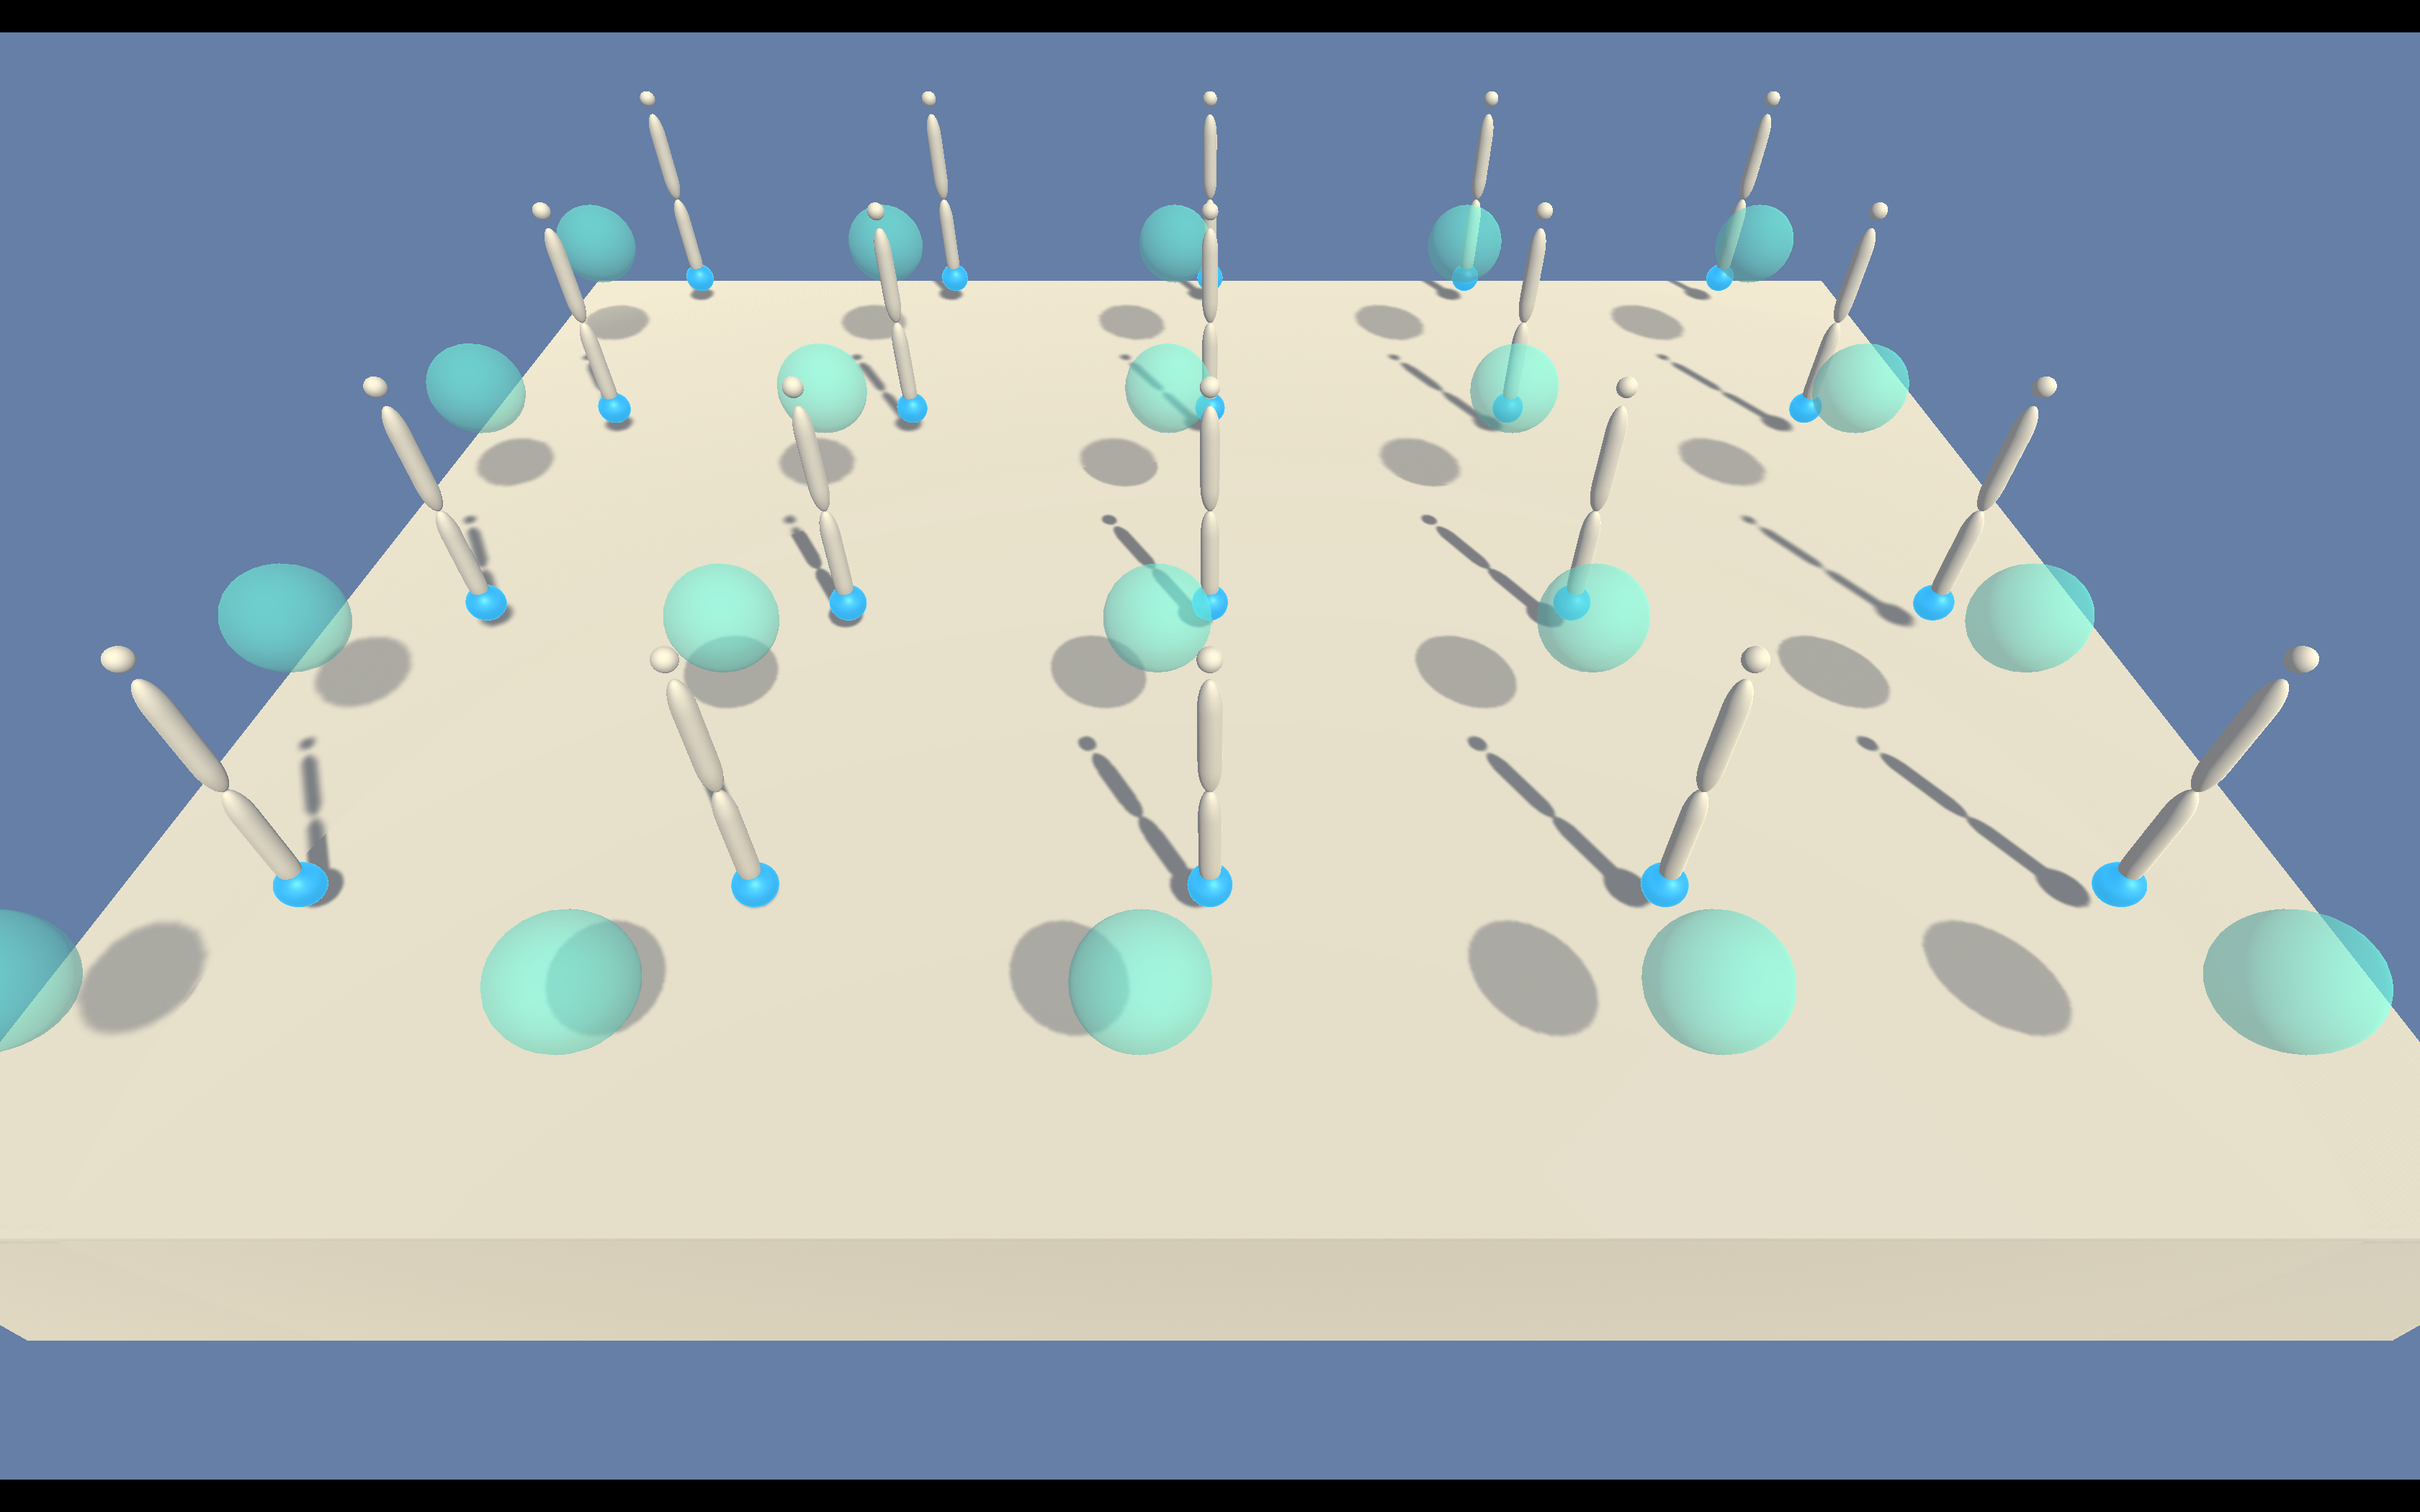
\includegraphics[width=\linewidth]{figures/envs/unity_reacher_20.png}
		\caption{3D Robotic Arm Unity Environment}
		\label{fig:unity_environment}
\end{figure}

\subsubsection{Observation Space}

The observation space of the environment consists of 26 variables corresponding to the position, rotation, velocity, and angular velocities of the two arm. In the following table~\ref{tab:unity_obs_space}, a full description for all the environment observation is provided.

\begin{table}[!htb]
		\centering
		\begin{tabular}{|c|l|l|c|}
				\hline
				\multicolumn{4}{|c|}{\textbf{Observation Space}}                                                                                                                                     \\ \hline
				\multicolumn{3}{|c|}{\textit{\textbf{Local Position of Central Arm}}} & \textit{X-Axis, Y-Axis, Z-Axis}                                                                          \\ \hline
				\multicolumn{3}{|c|}{\textit{\textbf{Rotation of Central Arm}}}      & \textit{X-Axis, Y-Axis, Z-Axis}                                                                          \\ \hline
				\multicolumn{3}{|c|}{\textit{\textbf{Central Arm Angular Velocity}}}               & \textit{\begin{tabular}[c]{@{}c@{}}how fast an object rotates\\  relative to another point\end{tabular}} \\ \hline
						\multicolumn{3}{|c|}{\textit{\textbf{Central Arm Velocity}}}                      & \textit{the speed of the arm}                                                                            \\ \hline
				\multicolumn{3}{|c|}{\textit{\textbf{Local Position of Elbow Arm}}} & \textit{X-Axis, Y-Axis, Z-Axis}                                                                          \\ \hline
				\multicolumn{3}{|c|}{\textit{\textbf{Rotation of Elbow Arm}}}      & \textit{X-Axis, Y-Axis, Z-Axis}                                                                          \\ \hline
				\multicolumn{3}{|c|}{\textit{\textbf{Elbow Arm Angular Velocity}}}               & \textit{\begin{tabular}[c]{@{}c@{}}how fast an object rotates\\  relative to another point\end{tabular}} \\ \hline
						\multicolumn{3}{|c|}{\textit{\textbf{Elbow Arm Velocity}}}                      & \textit{the speed of the arm}                                                                            \\ \hline
				\multicolumn{3}{|c|}{\textit{\textbf{Local Position of Target Goal}}}      & \textit{X-Axis, Y-Axis, Z-Axis}                                                                          \\ \hline
				\multicolumn{3}{|c|}{\textit{\textbf{Local Position of the arm hand}}}      & \textit{X-Axis, Y-Axis, Z-Axis}                                                                          \\ \hline
				\multicolumn{3}{|c|}{\textit{\textbf{The Goal Speed}}}                         & \textit{The speed of the target sphere}                                                                  \\ \hline
		\end{tabular}
		\caption{Unity 3-DOF Arm Observation Space}
		\label{tab:unity_obs_space}
\end{table}

\subsubsection{Action Space}

The action space of the environment is a continuous one in which it has a vector of 4 actions applied to the two joints which indicated the torque applied on the movement axes in the 3D space.


\begin{table}[!htb]
		\centering

		\begin{tabular}{|c|c|l|l|}
				\hline
				\multicolumn{4}{|c|}{\textbf{Action Space (Continuous)}}                                                    \\ \hline
				\multirow{2}{*}{\textbf{Center Joint Torques}}  & \multicolumn{3}{c|}{\textbf{torque X-axis: range(-1, 1)}} \\ \cline{2-4} 
																										& \multicolumn{3}{c|}{\textbf{torque Z-axis: range(-1, 1)}} \\ \hline
				\multirow{2}{*}{\textbf{Elbow Joint Torques}}   & \multicolumn{3}{c|}{\textbf{torque X-axis: range(-1, 1)}} \\ \cline{2-4} 
																										& \multicolumn{3}{c|}{\textbf{torque Z-axis: range(-1, 1)}} \\ \hline
		\end{tabular}
		\caption{Unity 3D Arm Actions Information}
		\label{tab:unity_arm_actions}

\end{table}

\subsubsection{Reward Function}

The reward function for this environment is different as we modify it to only give a reward of (+0.1) for the agent if the agent can reach the target sphere and keep moving with it along a circular path. Hence, the reward function is described as \textbf{\(R(\tau)=+0.1\)}.


\subsubsection{Experiment Results}

This experiment was performed in two different ways. The first time was training the agent from scratch to compare the performance of this environment with others performed in previous experiments. The second time is to try transfer learning trained agent from 2D environment to this 3D environment and watch the agent behaviour and the performance, whether the agent will perform as it is suppose to achieve the goal or it will need some more training to modify the policy and learn the right way to solve the environment. With this, we want to measure the time taken to continue training pre-trained agent to solve a new task.

$\bullet$ \textit{\textbf{First Trail: Training from scratch}} in this experiment, we trained the agents from scratch to observe the behaviour of training multiple agents inside one environment and to compare the training process of unity engine with openai gym (pybullet physics engine). 

The experiment is performed until an average reward of 35 achieved or for a maximum of 10000000 (10M) steps if no improvement is observable. For evaluating the model performance, we compare the average reward between both experiments. In total, we measure the following metrics averaging over each episode:
\begin{itemize}
		\item The Maximum reward the agent can achieve
		\item The Average reward the agent can achieve
		\item The Total Time Steps obtained by the agent
		\item The Total Time taken to perform the experiment
\end{itemize}

The maximum reward obtained in the environment is (750) reward for all the 20 agent, which means the single agent can obtain a maximum reward of (\~37.5) over the training process. The following figure~\ref{fig:4th_exp_max_eps_reward}, includes demonstration for the maximum reward obtained for the 20 multi-agents and the single agent with a comparison between all other agents in the previous experiments.
\begin{figure}[!htb]
		\centering
		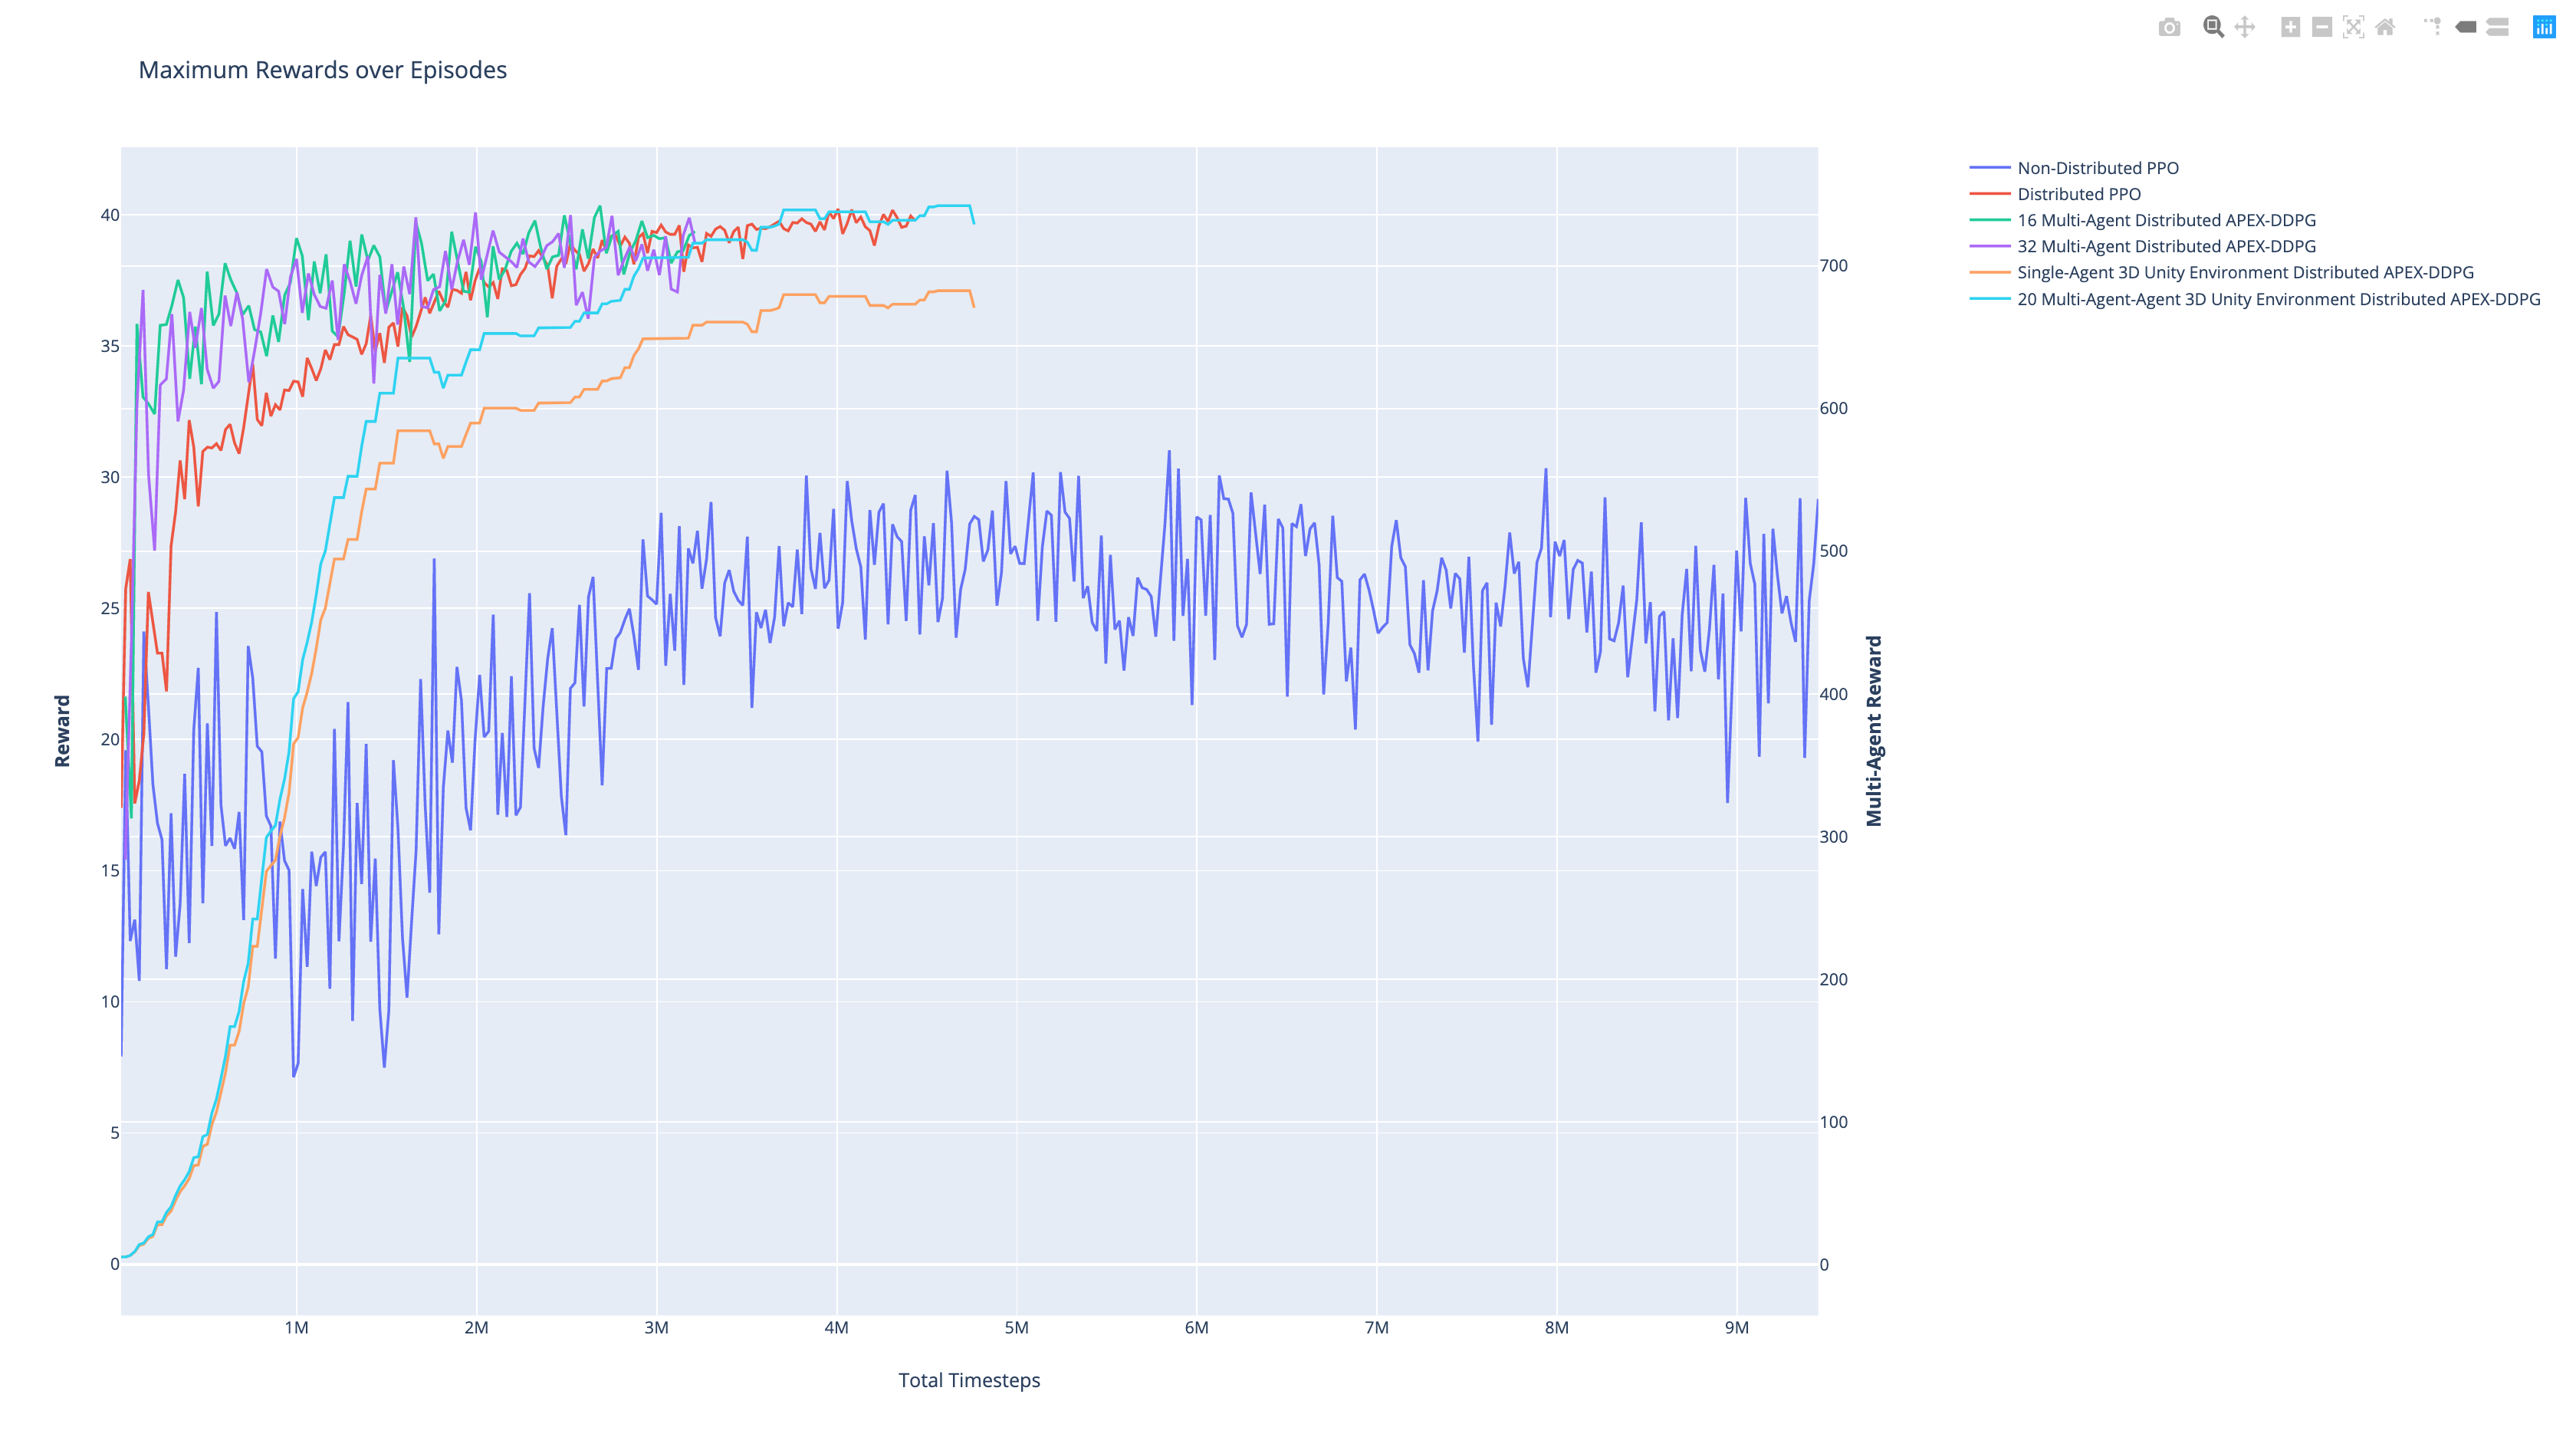
\includegraphics[width=\linewidth]{figures/exps/4th_exp/max_eps_reward.png}
		\caption[Maximum Reward over Episodes for the 5th distributed Ape-X DDPG experiment on Unity 3-DOF robotic arm]{Maximum Reward over Episodes for the 5th distributed Ape-X DDPG experiment on Unity 3-DOF robotic arm\footnotemark}
		\label{fig:4th_exp_max_eps_reward}
\end{figure}

For the average reward, the agents was able to obtain (700) reward in the environment after only 4M time-steps. This means a single agent obtain 35 reward and solved the required task after only 4M time-steps. The performance of these agent is similar to the distributed version of the PPO algorithm used in the second experiment. Following a figure~\ref{fig:4th_exp_avg_eps_reward} of the average reward for all the experiment.
\begin{figure}[!htb]
		\centering
		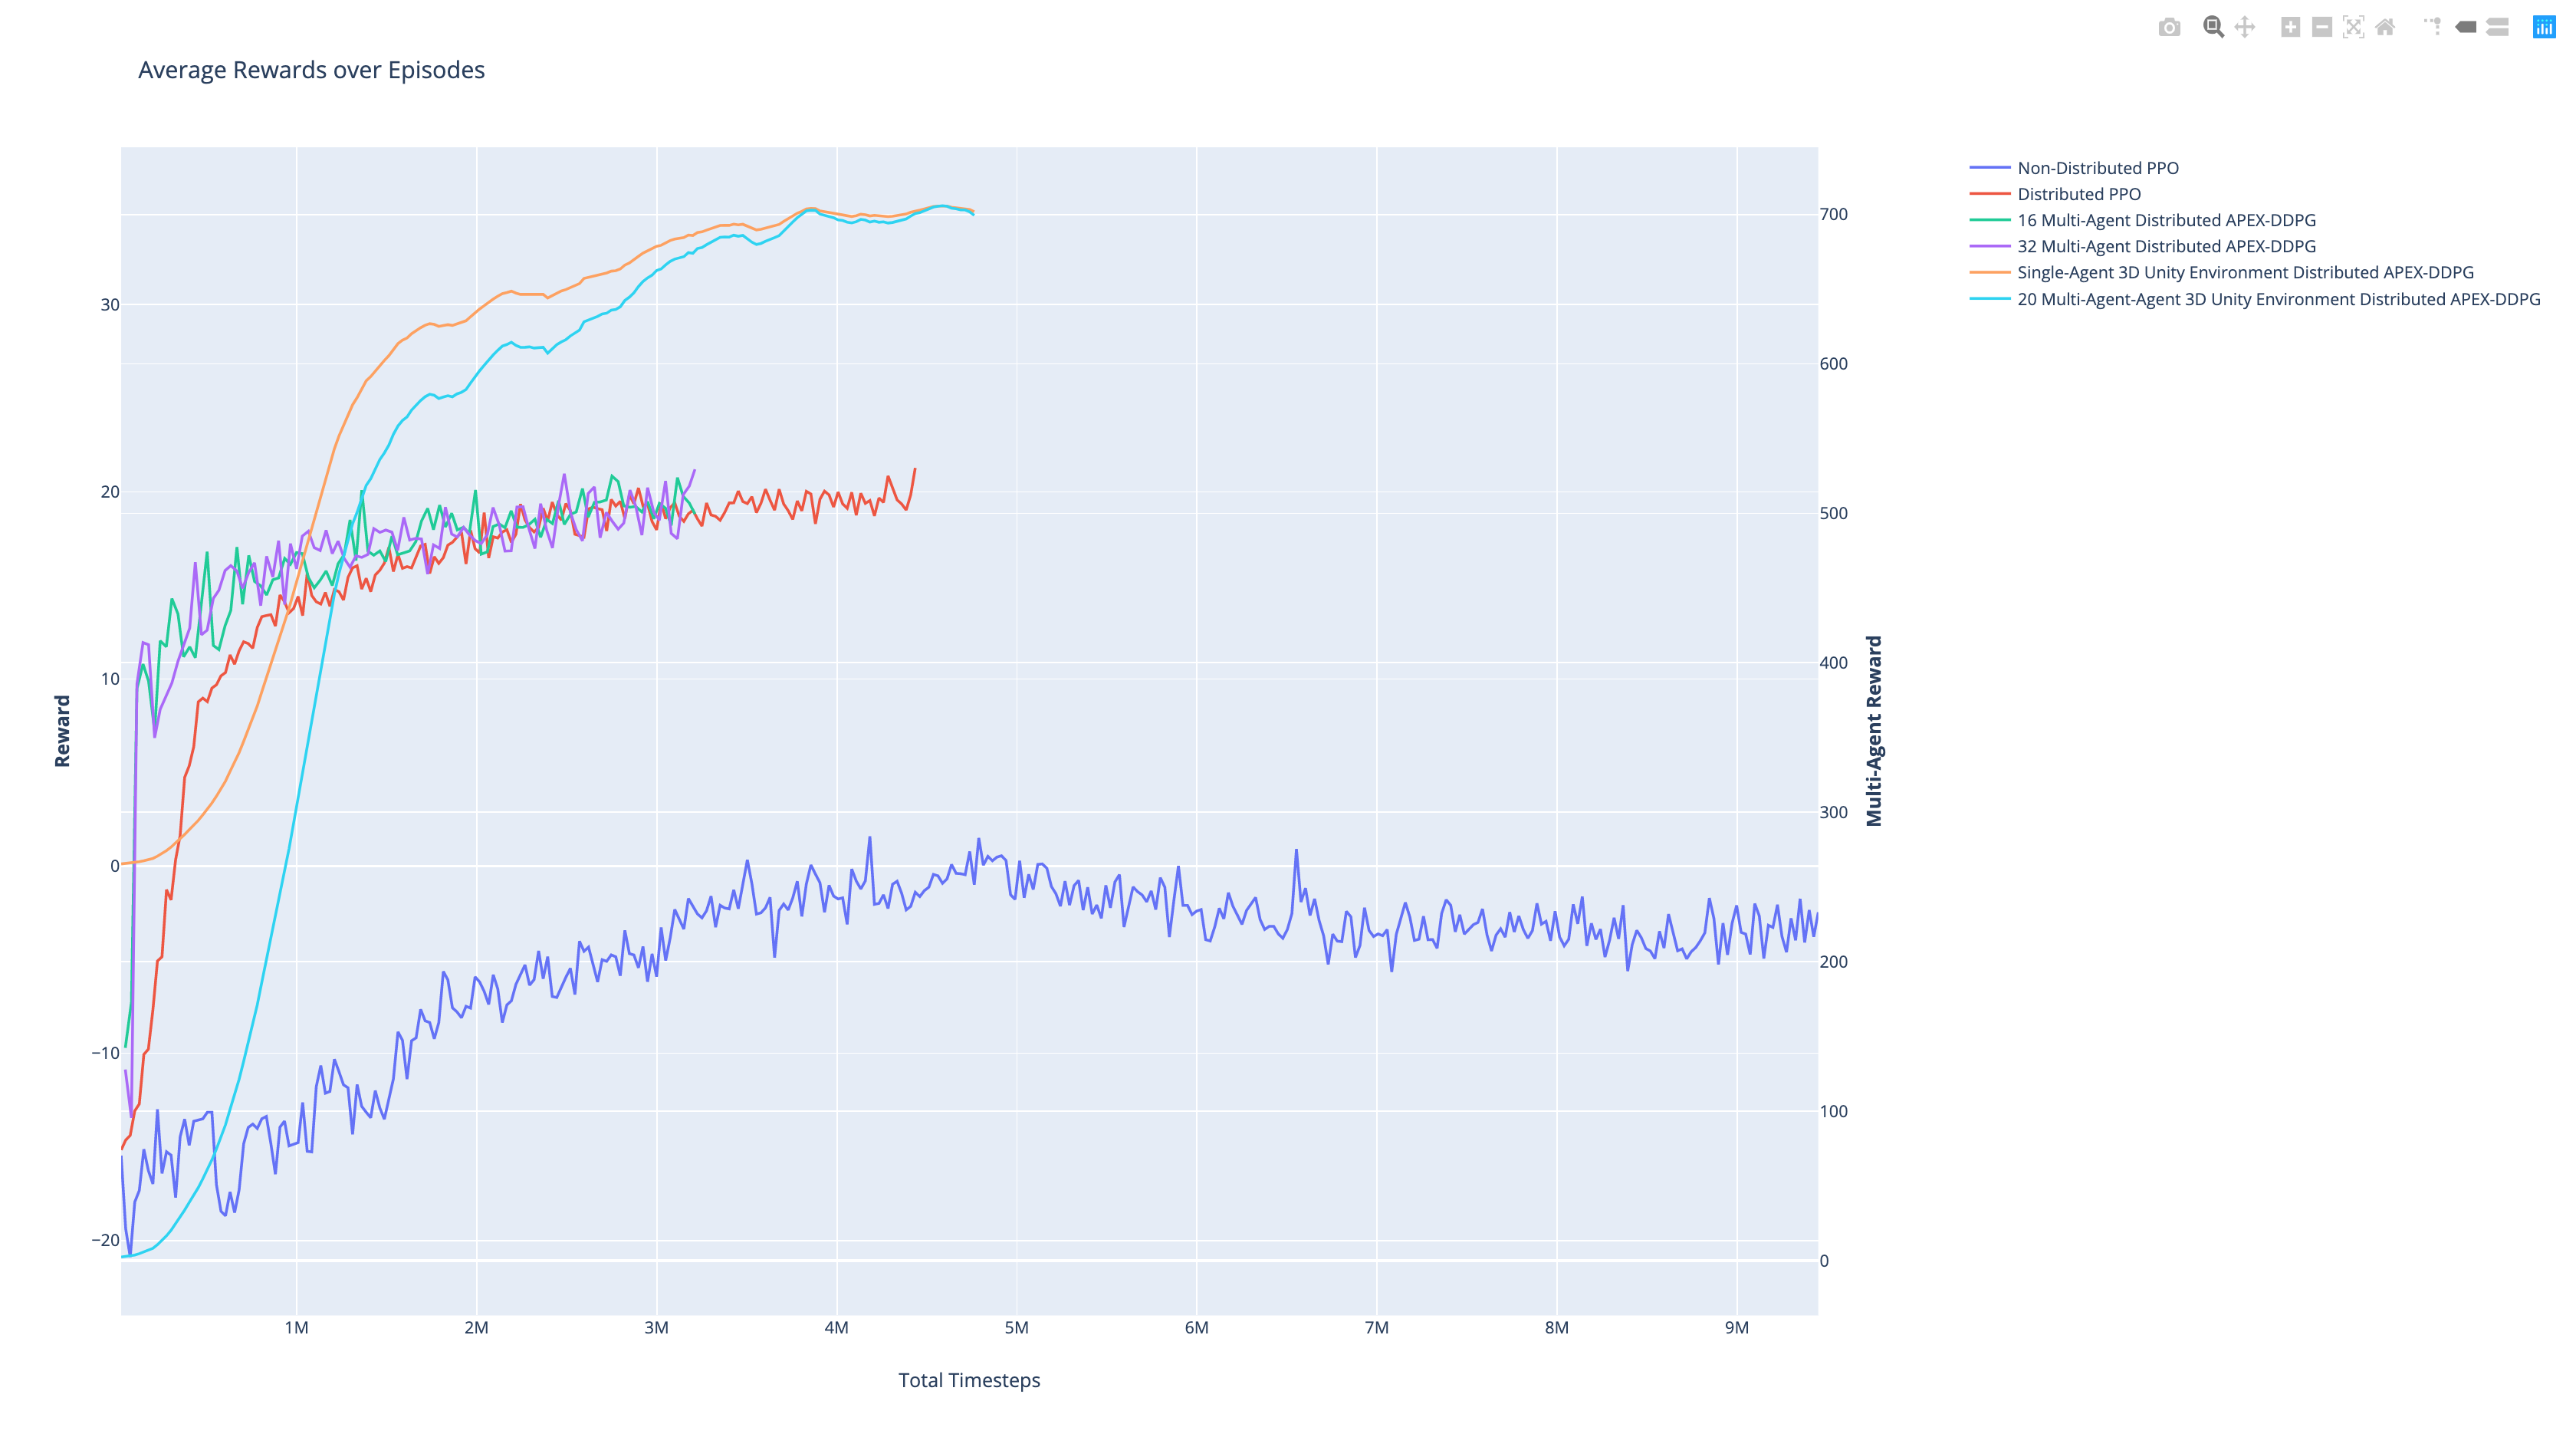
\includegraphics[width=\linewidth]{figures/exps/4th_exp/avg_eps_reward.png}
		\caption[Average Reward over Episodes for the 5th distributed Ape-X DDPG experiment on Unity 3-DOF robotic arm]{Average Reward over Episodes for the 5th distributed Ape-X DDPG experiment on Unity 3-DOF robotic arm\footnotemark}
		\label{fig:4th_exp_avg_eps_reward}
\end{figure}

Comparing between the experiment's total taken time, we found that the experiment took less than 2 Hours to solve the task and all the agent can achieve the required goal. This is also similar to the distributed version of the PPO algorithm in the second experiment. The total training time is shown below~\ref{fig:4th_exp_total_training_time}:
\begin{figure}[!htb]
		\centering
		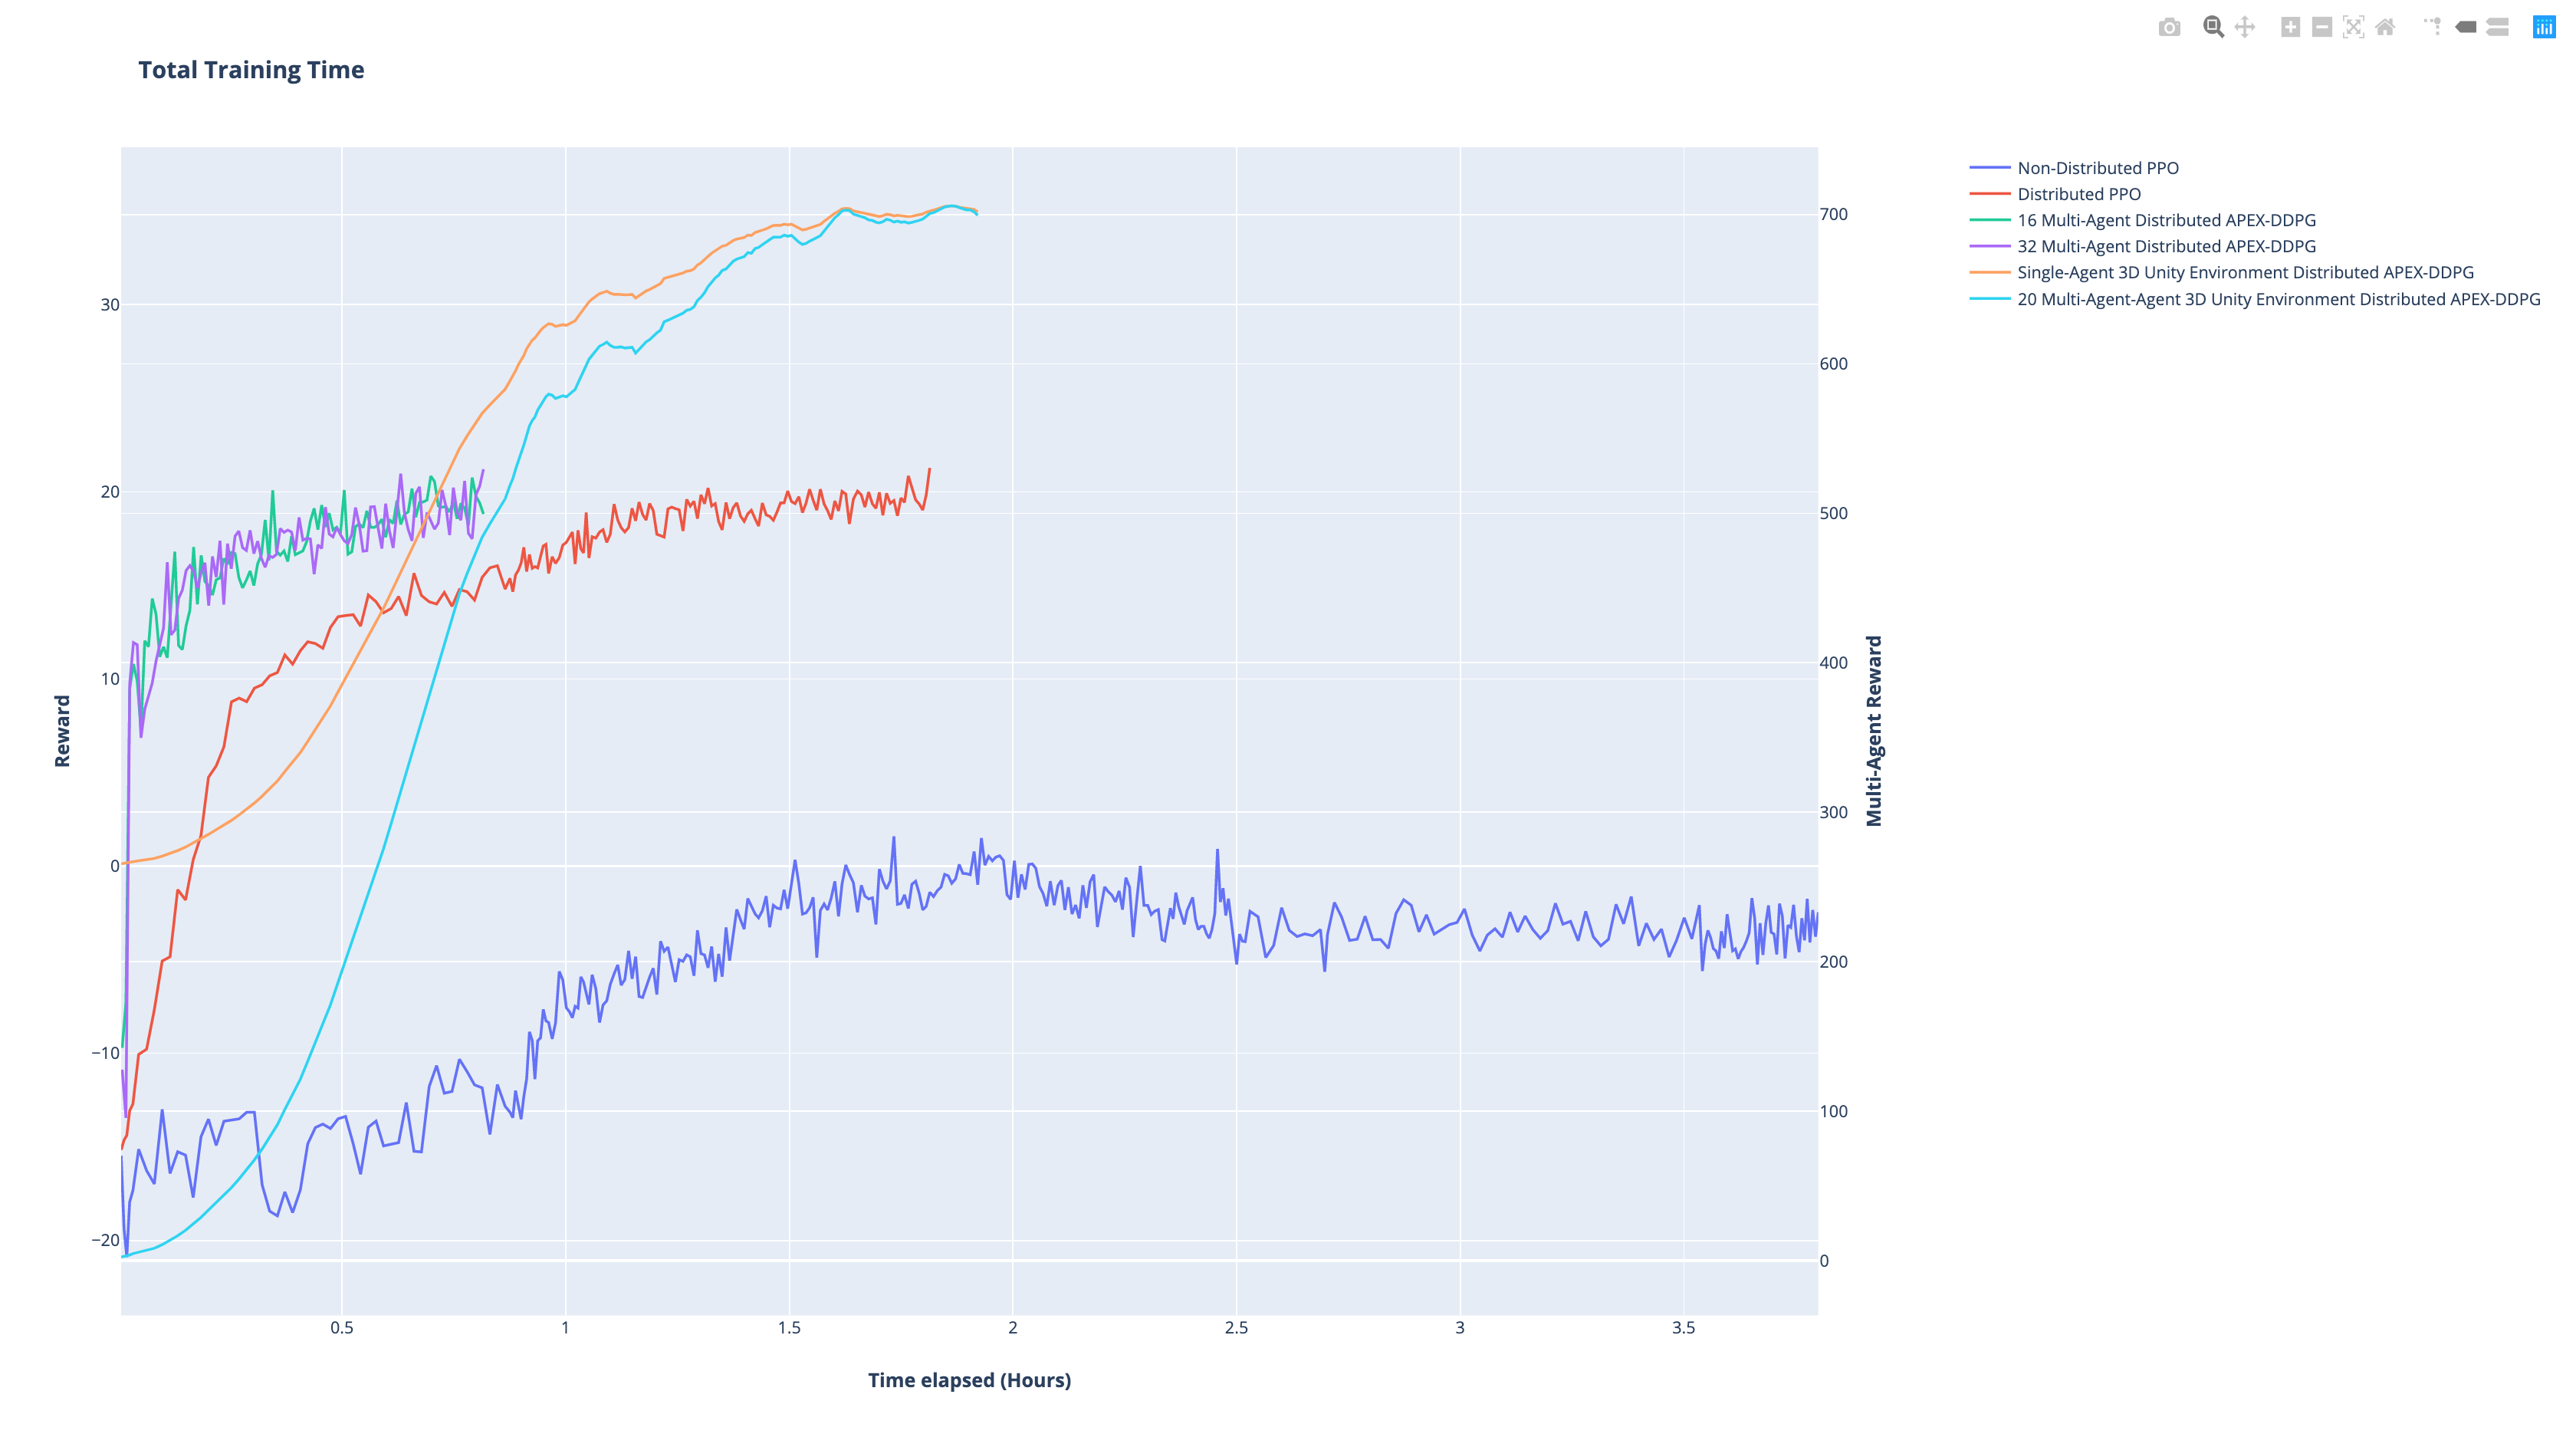
\includegraphics[width=\linewidth]{figures/exps/4th_exp/total_training_time.png}
		\caption[Total Training Time for the 5th distributed Ape-X DDPG experiment on Unity 3-DOF robotic arm]{Total Training Time for the 5th distributed Ape-X DDPG experiment on Unity 3-DOF robotic arm\footnotemark}
		\label{fig:4th_exp_total_training_time}
\end{figure}

\footnotetext{The blue line is identical to the red line indicating the reward obtained by single agent inside the environment.}

$\bullet$ \textit{\textbf{Second Trail: Transfer learning from gym trained agent}} in this experiment, the agent was trained on the previous environment with a modification for the neural network used to train the agent to share the same number of observation and action spaces. After training the agent, it was evaluated on the unity environment to observe how the agent will behave.

Based on the evaluation, shown in the figure~\ref{fig:4th_exp_1st_transfer_learning} below, the agent wasn't able to achieve any reward as shown in the figure below. This is because the agent was trained to output actions that are applied to the Y-axis in gym environment to be able to move the arm correctly. In contrast, unity environment applies the actions to X and Z axes for the arm.
\begin{figure}[!htb]
		\centering
		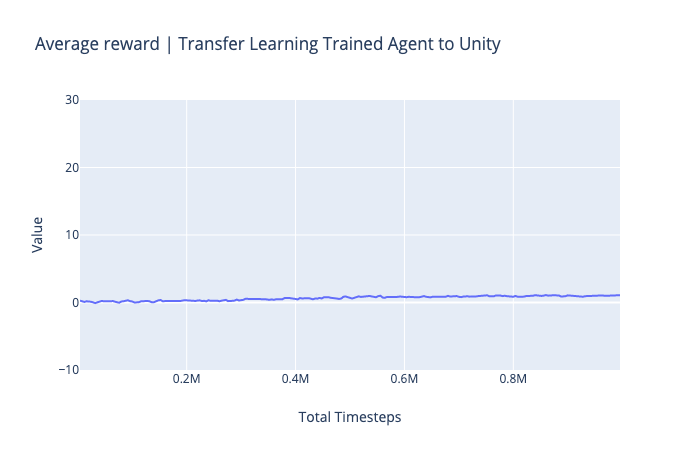
\includegraphics[width=\linewidth]{figures/exps/4th_exp/1st_transfer_learning.png}
		\caption{Average Reward of the first attempt of using Transfer Learning in the new unity environment.}
		\label{fig:4th_exp_1st_transfer_learning}
\end{figure}

In order to benefit from the trained agent, the experiment continue training the agent with unity environment and using the pre-trained weights and model from the gym trained agent to accelerate the training of the agent in the new environment. After only 17 minutes as shown in the figure~\ref{fig:4th_exp_2nd_transfer_learning} below, the agent was able to move the arm correctly and collect +25 reward based on the running evaluation on 1M time-steps.
\begin{figure}[!htb]
		\centering
		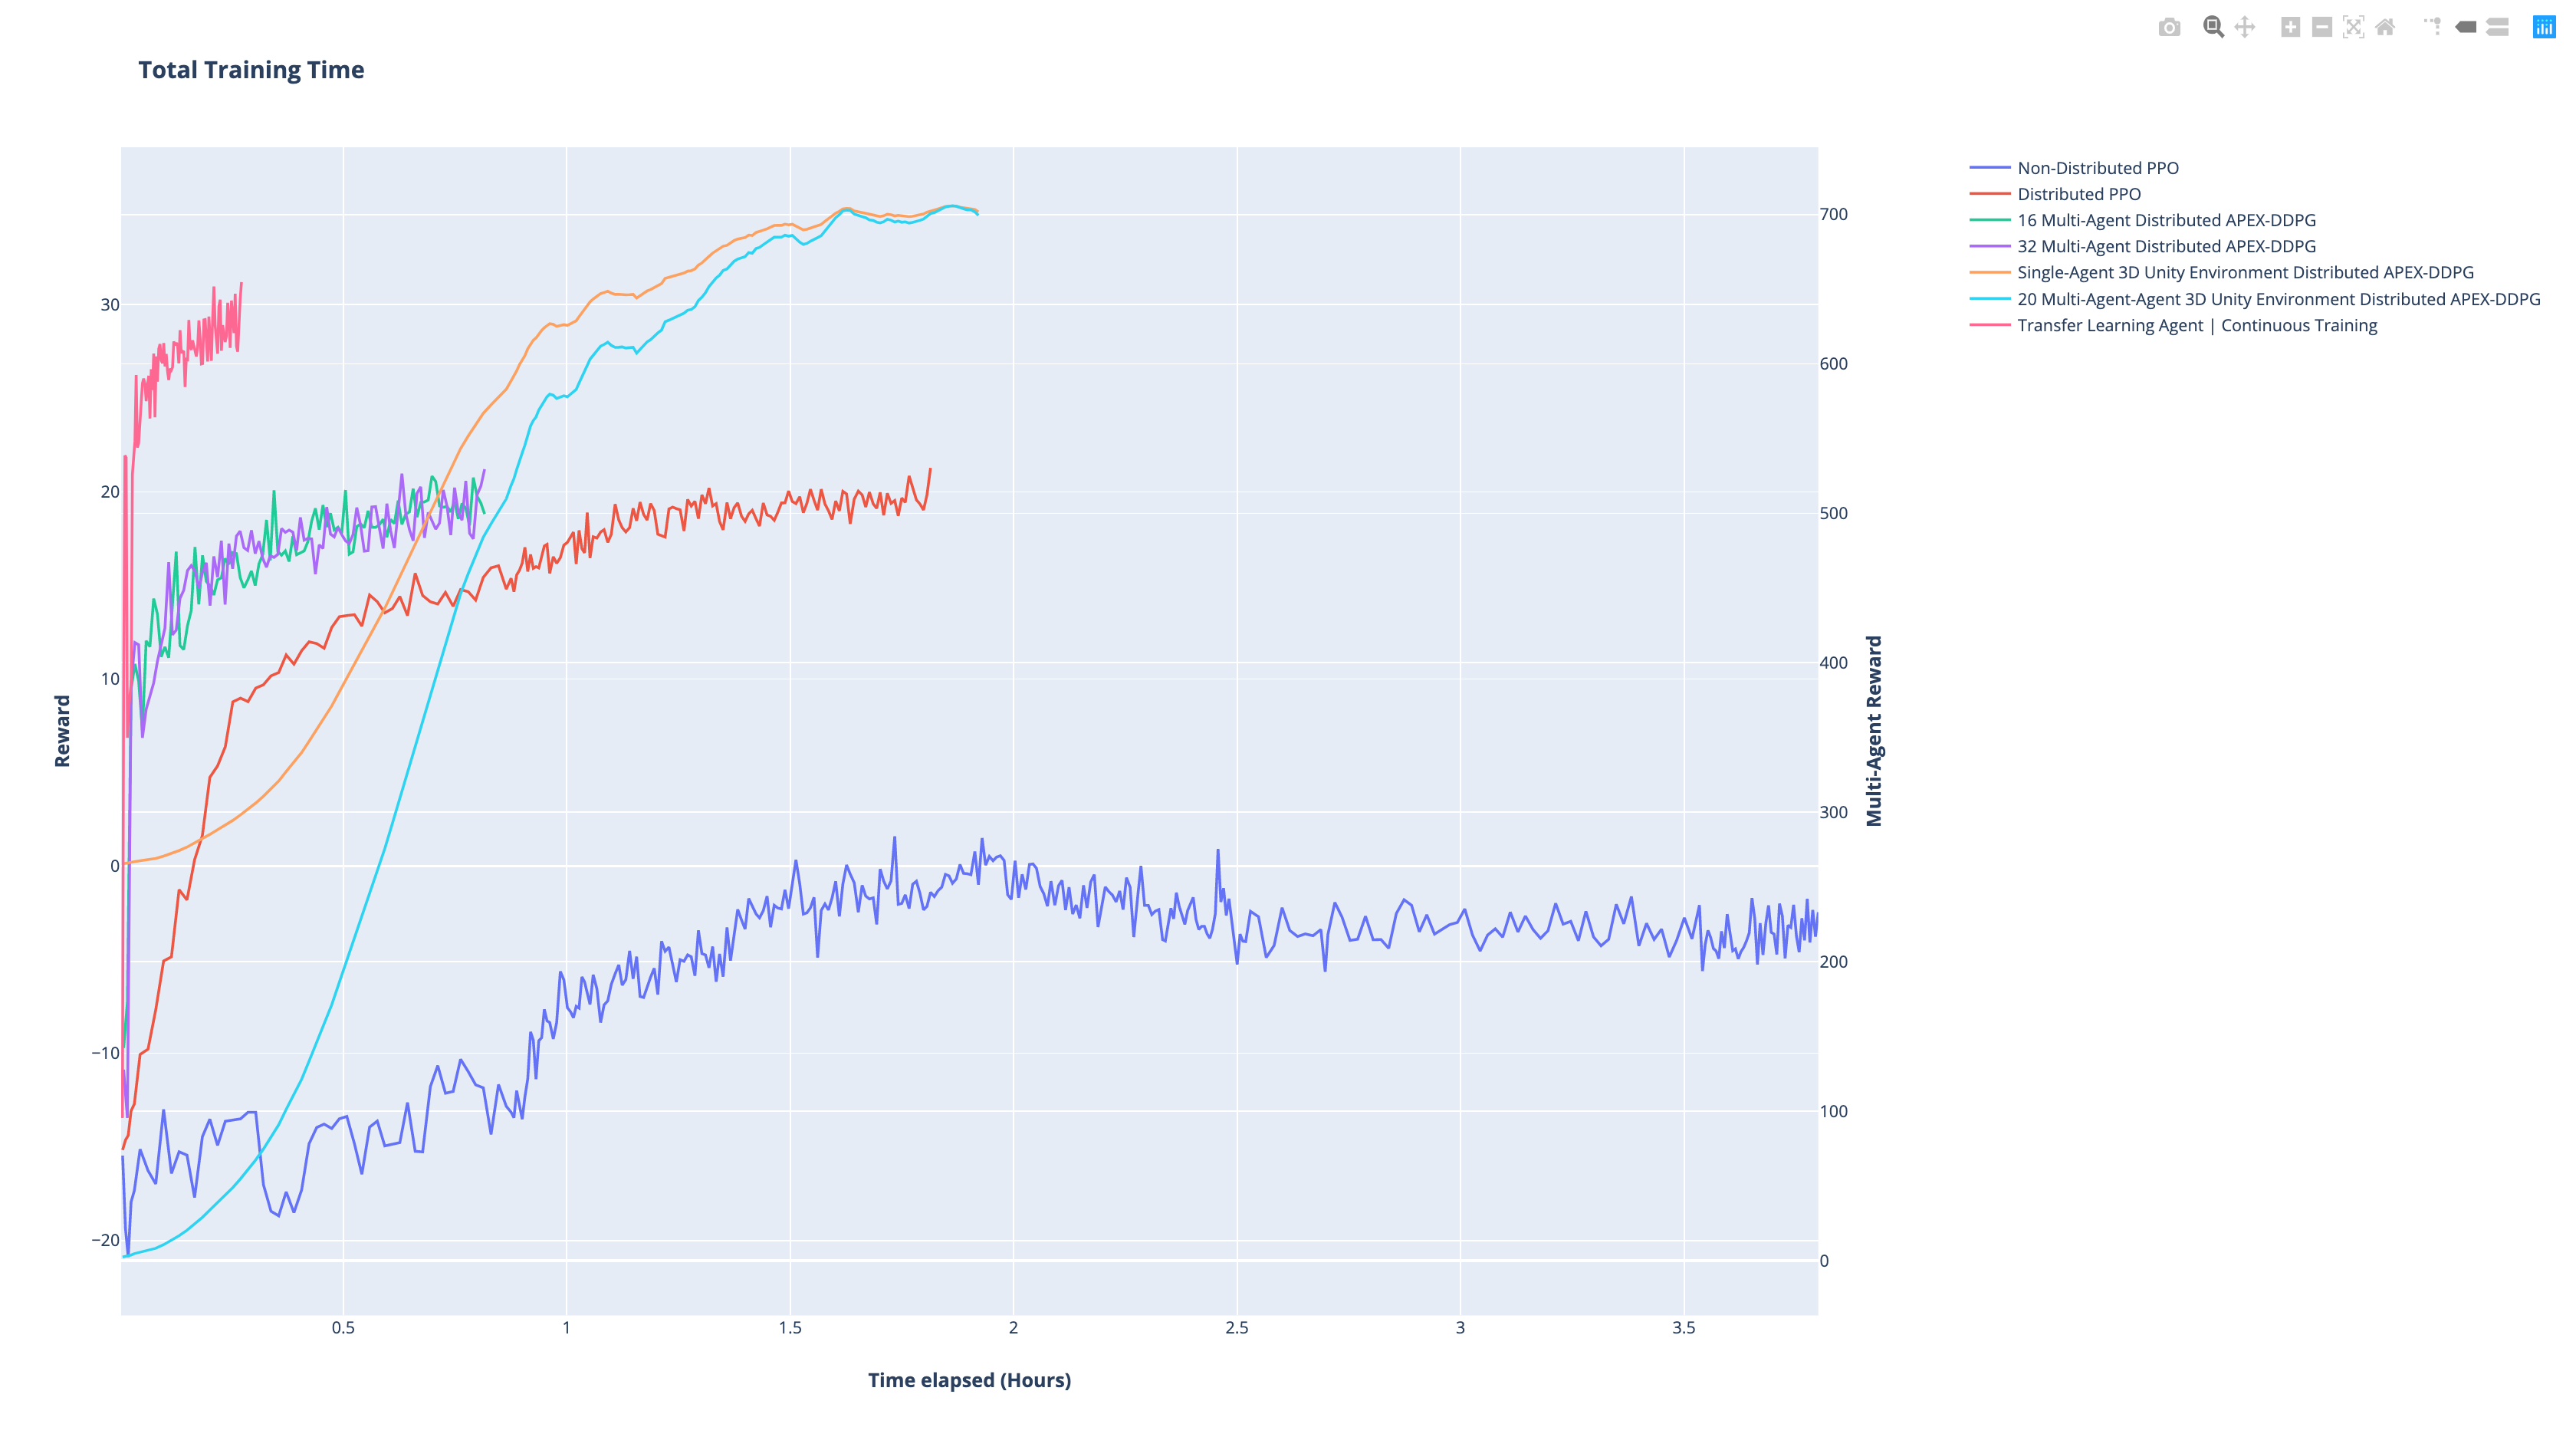
\includegraphics[width=\linewidth]{figures/exps/4th_exp/2nd_transfer_learning.png}
		\caption{Using Transfer Learning to continue training the pre-trained agent in the new 3D environment.}
		\label{fig:4th_exp_2nd_transfer_learning}
\end{figure}



\subsubsection{Conclusion}

In this experiment, a new 3D environment was used to train multiple agent inside one environment and test how to benefit from trained agent in 2D environment and use the weight and learned policy to learn a more complex policy and achieve the goal of the environment faster. The environment shows a similar performance as the distributed version of PPO in the second experiment. For transfer learning the agent wasn't able to solve the task from the first trail, instead it needed to be continue training and learning the new policy and in less than half an hour the agents was able to follow the target sphere and achieve 25 reward. Hence, it was possible to used pre-trained agent only after adjusting and continue learning in the new environment.